\documentclass[aspectratio=169,10pt]{beamer}

\usetheme{Madrid}
\usecolortheme{seahorse}

\usepackage{amsmath,amssymb,amsfonts}
\usepackage{mathtools}
\usepackage{bm}
\usepackage{graphicx}
\usepackage{booktabs}
\usepackage{listings}
\usepackage{xcolor}
\usepackage{algorithm}
\usepackage{algpseudocode}
\usepackage{tikz}
\usetikzlibrary{arrows.meta, positioning}

\graphicspath{{figures/}}

% Python listing style
\lstdefinestyle{pythonstyle}{
  language=Python,
  basicstyle=\ttfamily\scriptsize,
  numbers=left,
  numberstyle=\tiny\color{gray},
  frame=single,
  backgroundcolor=\color{gray!7},
  keywordstyle=\color{blue!70!black}\bfseries,
  stringstyle=\color{green!50!black},
  commentstyle=\color{gray!60}\itshape,
  showstringspaces=false,
  breaklines=true,
  tabsize=4,
  captionpos=b,
}
\lstset{style=pythonstyle}

\setbeamertemplate{footline}[frame number]
\setbeamertemplate{navigation symbols}{}

% ─── Title ────────────────────────────────────────────────────────────────────
\title[Ch.~19 Surrogate Optimization]{Chapter 19: Surrogate Optimization}
\subtitle{Algorithms for Optimization, 2nd Edition (2026)\\
          Kochenderfer \& Wheeler}
\author{Lecture Notes}
\date{2026}

% ══════════════════════════════════════════════════════════════════════════════
\begin{document}
% ══════════════════════════════════════════════════════════════════════════════

\begin{frame}
  \titlepage
\end{frame}

% ─── Table of Contents ────────────────────────────────────────────────────────
\begin{frame}{Chapter 19 Overview}
  \tableofcontents
\end{frame}

% ══════════════════════════════════════════════════════════════════════════════
\section{Introduction}
% ══════════════════════════════════════════════════════════════════════════════

\begin{frame}{Introduction: Why Surrogate Optimization?}
  \begin{columns}[T]
    \column{0.52\textwidth}
      \begin{block}{Motivation}
        \begin{itemize}
          \item Many real-world objective functions $f:\mathbb{R}^n\!\to\!\mathbb{R}$
                are \textbf{expensive} to evaluate (simulations, experiments).
          \item The previous chapter fitted a \textbf{Gaussian process (GP)}
                surrogate to infer Bayesian posterior predictive distributions
                over the true objective.
          \item Chapter 19 exploits these distributions to
                \emph{guide where to sample next}.
        \end{itemize}
      \end{block}
      \begin{alertblock}{Core Idea}
        Use the GP surrogate to balance \textbf{exploitation}
        (sample near the predicted minimum) and
        \textbf{exploration} (sample where uncertainty is high).
      \end{alertblock}
    \column{0.46\textwidth}
      \centering
      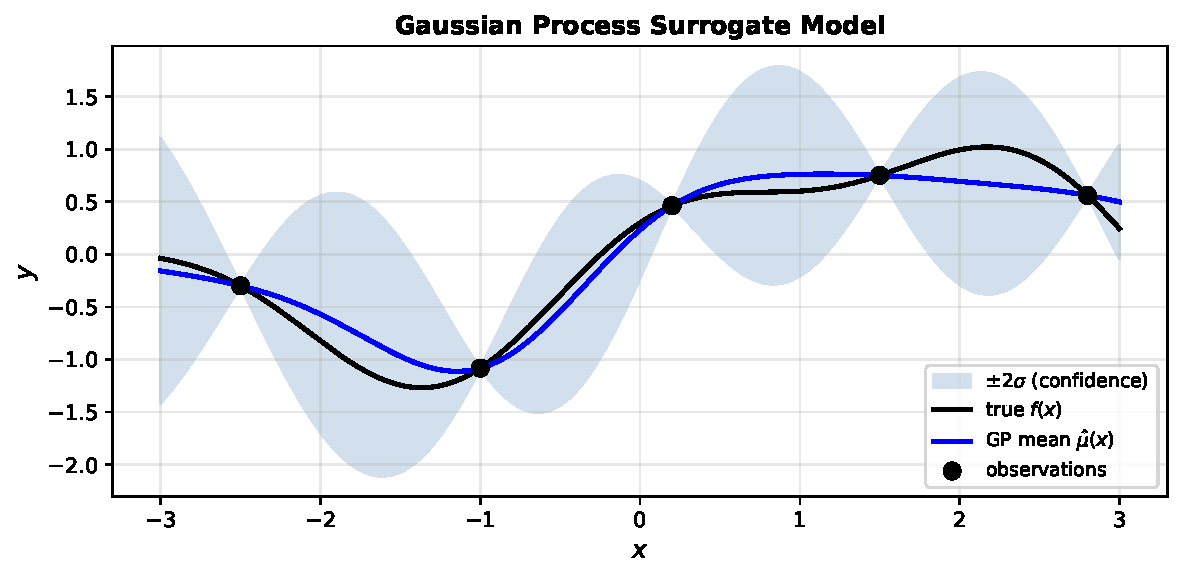
\includegraphics[width=\linewidth]{fig_gp_surrogate_overview}\\
      {\small GP surrogate $\hat{\mu}(x)$ with $\pm2\sigma$ confidence band
               fitted to black observations.}
  \end{columns}
\end{frame}

\begin{frame}{GP Surrogate: Key Quantities}
  \begin{columns}[T]
    \column{0.5\textwidth}
      At any unobserved point $\mathbf{x}$, the GP provides:
      \begin{block}{Predictive Mean}
        $\hat{\mu}(\mathbf{x})$ — best estimate of $f(\mathbf{x})$
      \end{block}
      \begin{block}{Predictive Standard Deviation}
        $\hat{\sigma}(\mathbf{x})$ — uncertainty about $f(\mathbf{x})$
      \end{block}
      \vspace{0.4em}
      \textbf{Bayesian framework:}
      \[
        f(\mathbf{x}) \mid \text{data} \;\sim\;
        \mathcal{N}\!\bigl(\hat{\mu}(\mathbf{x}),\,\hat{\sigma}^2(\mathbf{x})\bigr)
      \]
      \vspace{0.4em}
      \begin{itemize}
        \item Large $\hat{\sigma}$ $\Rightarrow$ high uncertainty $\Rightarrow$ explore.
        \item Small $\hat{\mu}$ $\Rightarrow$ promising region $\Rightarrow$ exploit.
      \end{itemize}
    \column{0.48\textwidth}
      \begin{block}{Exploration Strategies Covered}
        \begin{enumerate}
          \item Prediction-based exploration
          \item Error-based exploration
          \item Lower Confidence Bound (LCB/UCB)
          \item Probability of Improvement (PoI)
          \item Expected Improvement (EI)
          \item Safe Optimization (SafeOpt)
        \end{enumerate}
      \end{block}
  \end{columns}
\end{frame}

% ══════════════════════════════════════════════════════════════════════════════
\section{Prediction-Based Exploration}
% ══════════════════════════════════════════════════════════════════════════════

\begin{frame}{19.1 Prediction-Based Exploration}
  \begin{columns}[T]
    \column{0.52\textwidth}
      \begin{block}{Strategy}
        Select the next design point by \textbf{minimizing the predicted mean}
        of the surrogate:
        \[
          \mathbf{x}^{(m+1)} = \arg\min_{\mathbf{x}} \hat{\mu}(\mathbf{x})
          \tag{19.1}
        \]
      \end{block}
      \begin{itemize}
        \item Pure \textbf{exploitation}: always samples where GP thinks
              the minimum is.
        \item Simple, but can get \textbf{stuck} at a single point if the
              GP mean has a single global minimizer.
        \item \textbf{Failure mode:} With a zero-mean GP and a single sample
              $\mathbf{x}^{(1)}$, the predicted mean has a single global minimizer
              at $\mathbf{x}^{(1)}$ — the method will keep sampling the same point.
      \end{itemize}
    \column{0.46\textwidth}
      \centering
      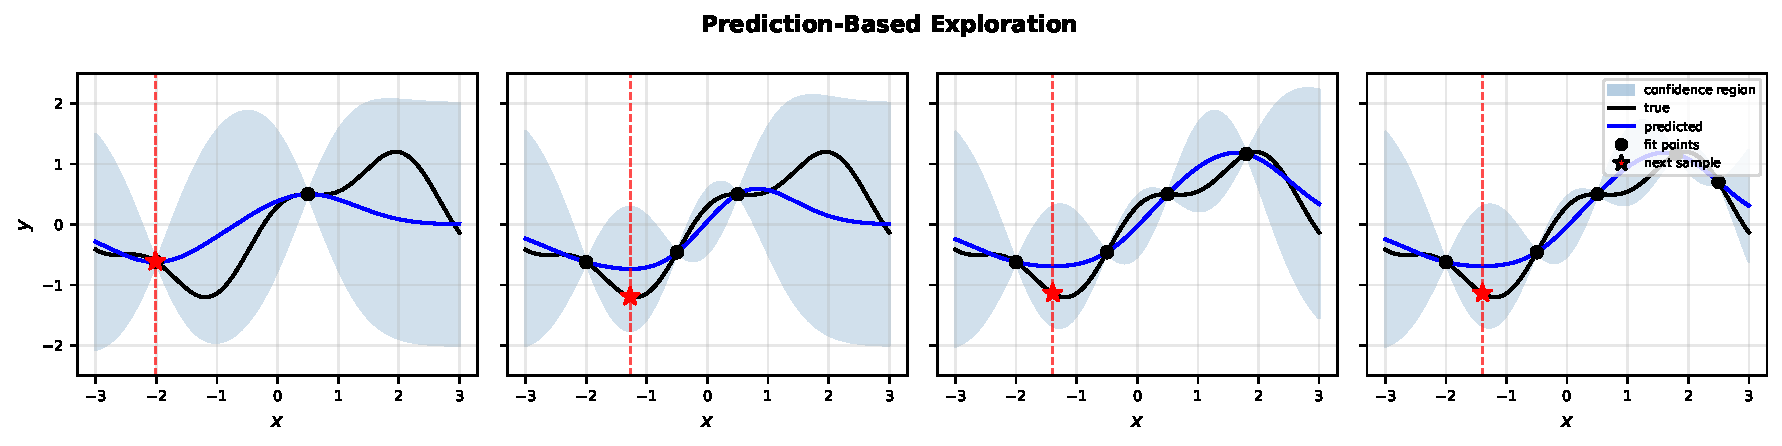
\includegraphics[width=\linewidth]{fig_prediction_based}\\
      {\small Four iterations of prediction-based exploration.
               Red star = next sample = $\arg\min \hat{\mu}$.}
  \end{columns}
\end{frame}

\begin{frame}[fragile]{Prediction-Based Exploration: Python Implementation}
\begin{lstlisting}[caption={Prediction-based surrogate optimization in Python}]
import numpy as np
from scipy.optimize import minimize
from sklearn.gaussian_process import GaussianProcessRegressor
from sklearn.gaussian_process.kernels import RBF, ConstantKernel

def prediction_based_optimization(f, bounds, n_init=3, n_iter=10):
    """
    Prediction-based (pure exploitation) surrogate optimization.
    f      : expensive objective function  f: R^n -> R
    bounds : list of (lo, hi) per dimension
    """
    dim = len(bounds)
    # Initial random samples
    lo = np.array([b[0] for b in bounds])
    hi = np.array([b[1] for b in bounds])
    X = lo + np.random.rand(n_init, dim) * (hi - lo)
    y = np.array([f(x) for x in X])

    kernel = ConstantKernel(1.0) * RBF(length_scale=1.0)
    gp = GaussianProcessRegressor(kernel=kernel, n_restarts_optimizer=5,
                                   normalize_y=True)
    for _ in range(n_iter):
        gp.fit(X, y)

        # Minimize predicted mean  (equation 19.1)
        best = None
        for x0 in X[np.argsort(y)[:3]]:  # warm start from best known
            res = minimize(lambda x: gp.predict(x.reshape(1,-1))[0],
                           x0, bounds=bounds, method='L-BFGS-B')
            if best is None or res.fun < best.fun:
                best = res

        x_new = np.clip(best.x, lo, hi)
        y_new = f(x_new)
        X = np.vstack([X, x_new])
        y = np.append(y, y_new)

    best_idx = np.argmin(y)
    return X[best_idx], y[best_idx]

# Example usage
f = lambda x: np.sin(x[0]) + 0.3 * np.cos(3*x[0])
x_opt, y_opt = prediction_based_optimization(f, [(-3, 3)])
print(f"Best x={x_opt[0]:.4f},  f(x)={y_opt:.4f}")
\end{lstlisting}
\end{frame}

% ══════════════════════════════════════════════════════════════════════════════
\section{Error-Based Exploration}
% ══════════════════════════════════════════════════════════════════════════════

\begin{frame}{19.2 Error-Based Exploration}
  \begin{columns}[T]
    \column{0.52\textwidth}
      \begin{block}{Strategy}
        Select the next design point where the GP has the
        \textbf{highest uncertainty} (maximum standard deviation):
        \[
          \mathbf{x}^{(m+1)} = \arg\max_{\mathbf{x}} \hat{\sigma}(\mathbf{x})
          \tag{19.2}
        \]
      \end{block}
      \begin{itemize}
        \item Pure \textbf{exploration}: fills in gaps in the input space.
        \item Ignores the objective function values — does \emph{not}
              try to minimize $f$.
        \item \textbf{Problem:} GP with unbounded domain always has high
              uncertainty far from samples, pulling exploration away from
              the region of interest.
        \item \textbf{Fix:} Constrain exploration to a \emph{closed region}.
      \end{itemize}
    \column{0.46\textwidth}
      \centering
      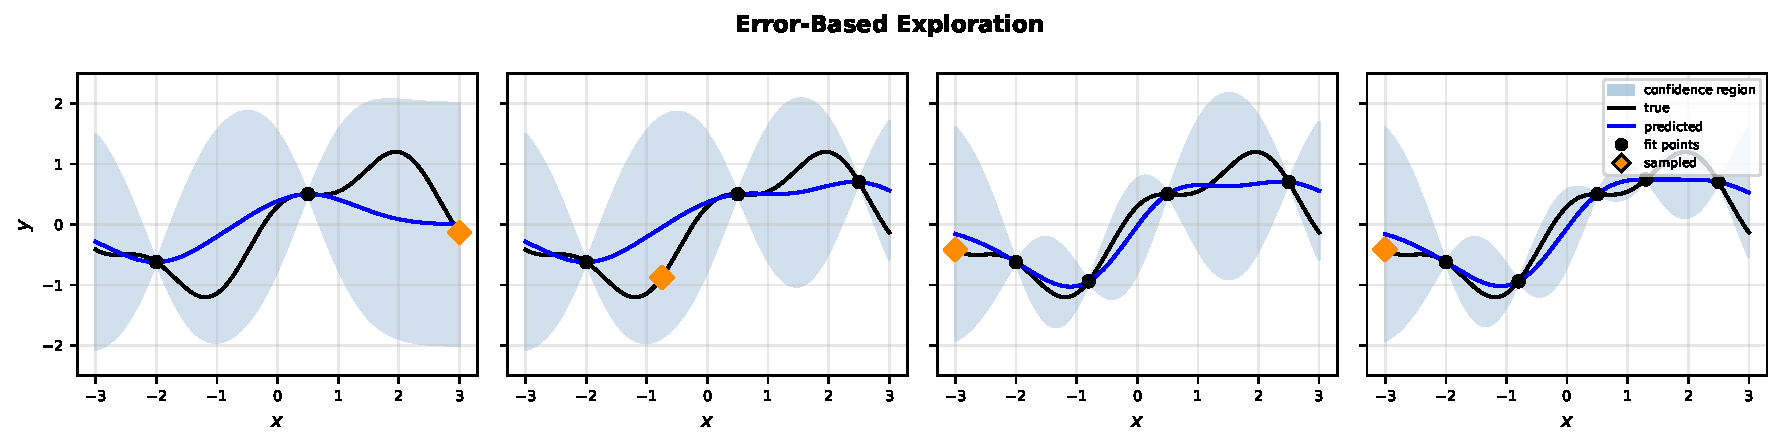
\includegraphics[width=\linewidth]{fig_error_based}\\
      {\small Orange diamond = next sample = $\arg\max \hat{\sigma}$.
               Samples fill the input space uniformly.}
  \end{columns}
\end{frame}

% ══════════════════════════════════════════════════════════════════════════════
\section{Lower Confidence Bound (UCB)}
% ══════════════════════════════════════════════════════════════════════════════

\begin{frame}{19.3 Lower Confidence Bound (LCB) Exploration}
  \begin{columns}[T]
    \column{0.56\textwidth}
      \begin{block}{The LCB Acquisition Function}
        Combine prediction and uncertainty by sampling the point
        that minimizes the \textbf{lower confidence bound}:
        \[
          \mathbf{x}^{(m+1)} = \arg\min_{\mathbf{x}}
          \bigl[\hat{\mu}(\mathbf{x}) - \alpha\,\hat{\sigma}(\mathbf{x})\bigr]
          \tag{19.3}
        \]
        where $\alpha > 0$ is a \textbf{trade-off scalar}.
      \end{block}
      \medskip
      \textbf{Symbol glossary:}
      \begin{itemize}
        \item $\hat{\mu}(\mathbf{x})$ — GP predicted mean at $\mathbf{x}$
        \item $\hat{\sigma}(\mathbf{x})$ — GP predicted std.\ deviation at $\mathbf{x}$
        \item $\alpha$ — exploration weight ($\alpha \uparrow$ $\Rightarrow$ more exploration)
      \end{itemize}
      \begin{exampleblock}{Interpretation}
        \begin{itemize}
          \item $\alpha = 0$: reduces to prediction-based (pure exploitation).
          \item Large $\alpha$: favours uncertain regions (exploration).
          \item \textbf{Bridges} the exploitation--exploration trade-off.
        \end{itemize}
      \end{exampleblock}
    \column{0.42\textwidth}
      \centering
      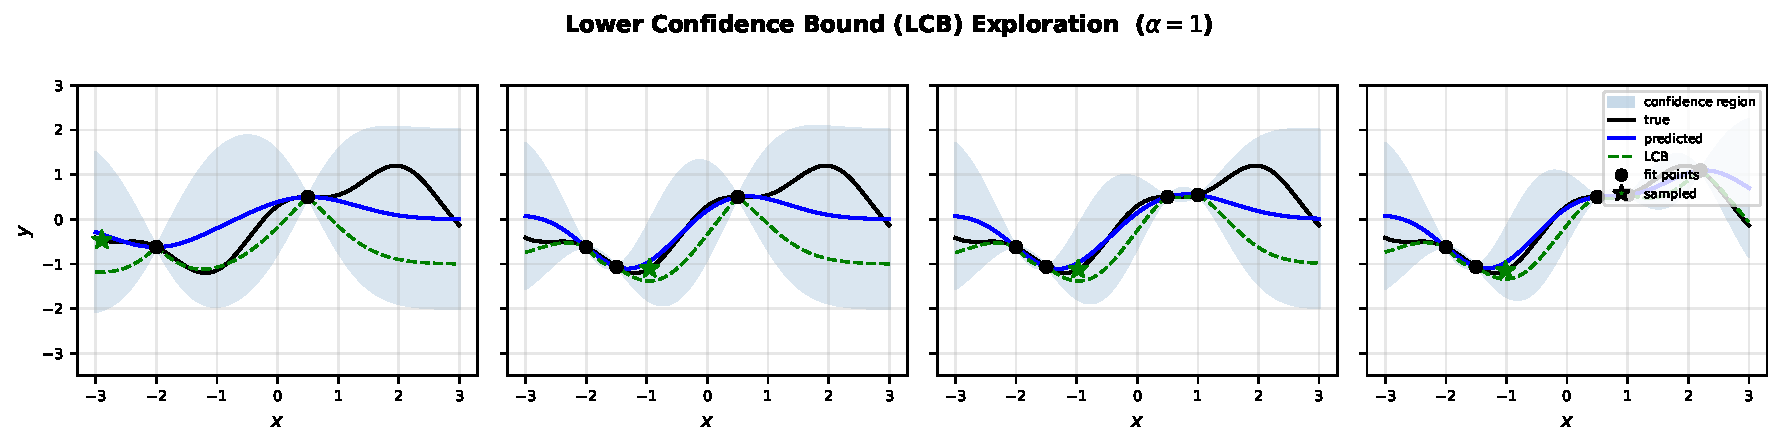
\includegraphics[width=\linewidth]{fig_lcb}\\
      {\small Green dashed = LCB$= \hat{\mu} - \alpha\hat{\sigma}$.
               Green star = $\arg\min$ LCB.}
  \end{columns}
\end{frame}

\begin{frame}[fragile]{LCB Exploration: Python}
\begin{lstlisting}[caption={Lower Confidence Bound acquisition function (Python)}]
import numpy as np
from scipy.optimize import differential_evolution
from sklearn.gaussian_process import GaussianProcessRegressor
from sklearn.gaussian_process.kernels import RBF, ConstantKernel

def lcb_optimization(f, bounds, alpha=1.0, n_init=3, n_iter=15):
    """
    Bayesian optimization with Lower Confidence Bound acquisition.
    Parameters
    ----------
    alpha : float
        Exploration weight. Higher alpha => more exploration.
    """
    dim = len(bounds)
    lo = np.array([b[0] for b in bounds])
    hi = np.array([b[1] for b in bounds])
    X = lo + np.random.rand(n_init, dim) * (hi - lo)
    y = np.array([f(x) for x in X])

    kernel = ConstantKernel(1.0) * RBF(length_scale=1.0)
    gp = GaussianProcessRegressor(kernel=kernel, n_restarts_optimizer=5,
                                   normalize_y=True)
    for k in range(n_iter):
        gp.fit(X, y)

        # LCB acquisition: minimize  mu - alpha * sigma  (Eq. 19.3)
        def lcb(x):
            x = np.array(x).reshape(1, -1)
            mu, sigma = gp.predict(x, return_std=True)
            return float(mu - alpha * sigma)

        res = differential_evolution(lcb, bounds, seed=42, tol=1e-6)
        x_new = np.clip(res.x, lo, hi)
        X = np.vstack([X, x_new])
        y = np.append(y, f(x_new))

    best_idx = np.argmin(y)
    return X[best_idx], y[best_idx]

# Numerical example: minimize f(x) = sin(x) + 0.3*cos(3x) on [-3, 3]
f = lambda x: np.sin(x[0]) + 0.3 * np.cos(3 * x[0])
x_opt, y_opt = lcb_optimization(f, [(-3.0, 3.0)], alpha=1.0, n_iter=12)
print(f"LCB optimum: x = {x_opt[0]:.4f},  f(x) = {y_opt:.4f}")
\end{lstlisting}
\end{frame}

% ══════════════════════════════════════════════════════════════════════════════
\section{Probability of Improvement}
% ══════════════════════════════════════════════════════════════════════════════

\begin{frame}{19.4 Probability of Improvement (PoI)}
  \begin{columns}[T]
    \column{0.54\textwidth}
      \begin{block}{Improvement Function}
        Define the improvement at a point $\mathbf{x}$ as:
        \[
          I(y) = \max(y_{\min} - y,\; 0)
          \tag{19.4}
        \]
        where $y_{\min}$ is the \textbf{best value sampled so far}.
      \end{block}
      \begin{block}{Probability of Improvement (PoI)}
        For $\hat{\sigma} > 0$, the PoI is:
        \[
          P(y < y_{\min}) = \int_{-\infty}^{y_{\min}}
            \mathcal{N}(y \mid \hat{\mu}, \hat{\sigma}^2)\,dy
          \tag{19.5}
        \]
        \[
          = \Phi\!\left(\frac{y_{\min} - \hat{\mu}}{\hat{\sigma}}\right)
          \tag{19.6}
        \]
      \end{block}
      \medskip
      \textbf{Symbol glossary:}
      \begin{itemize}
        \item $y_{\min}$ — current best observed value
        \item $\hat{\mu}, \hat{\sigma}$ — GP posterior mean \& std at $\mathbf{x}$
        \item $\Phi$ — standard normal CDF
      \end{itemize}
    \column{0.44\textwidth}
      \centering
      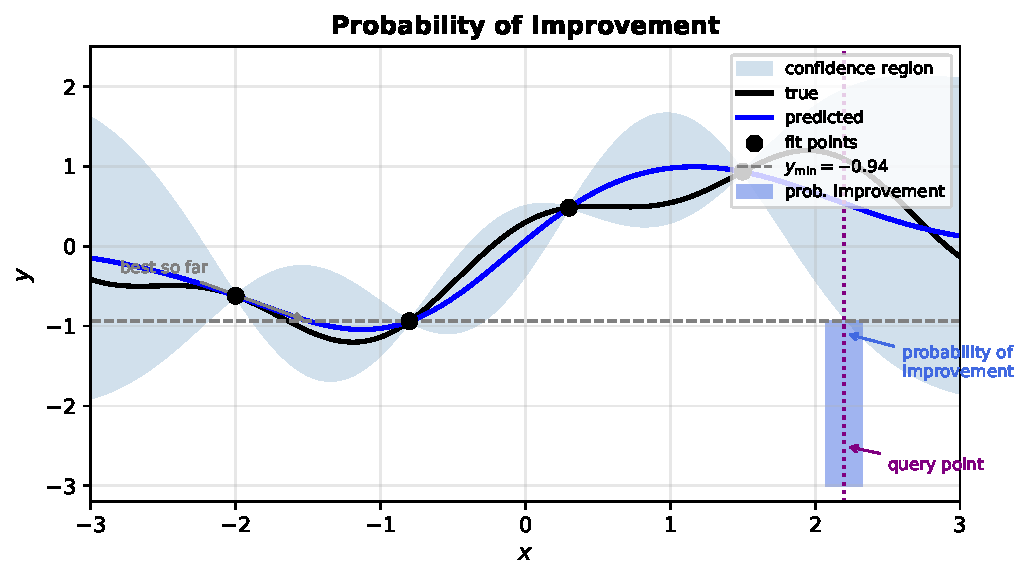
\includegraphics[width=\linewidth]{fig_prob_improvement}\\
      {\small Shaded blue region below $y_{\min}$ at the query point
               is the probability of improvement.}
  \end{columns}
\end{frame}

\begin{frame}{PoI: Progression Across Iterations}
  \centering
  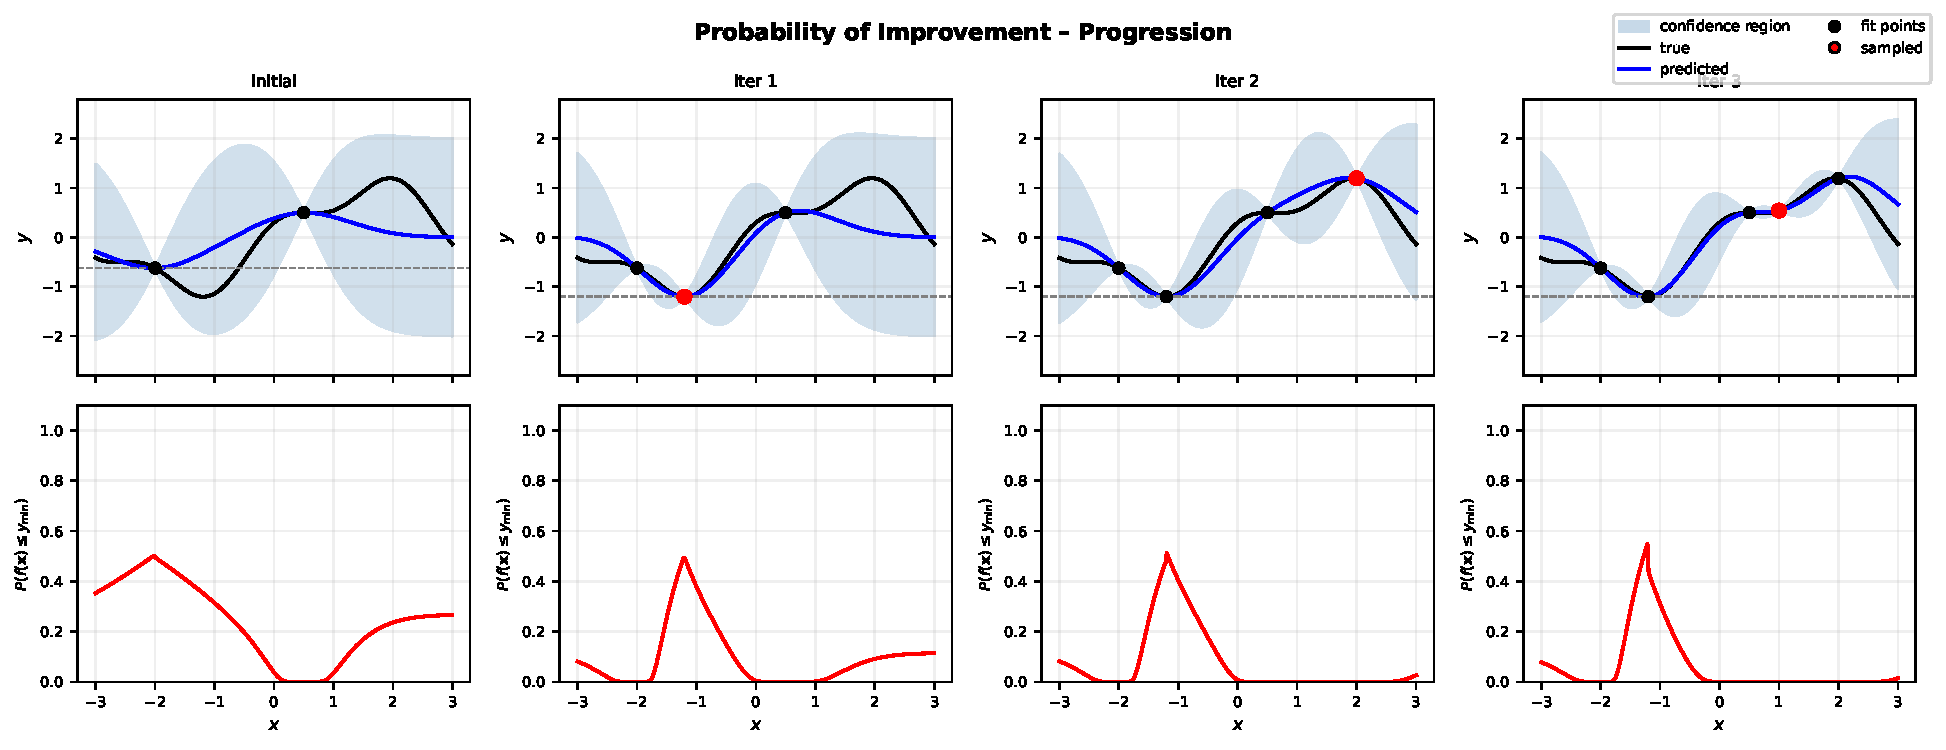
\includegraphics[width=0.95\linewidth]{fig_poi_progression}
  \vspace{0.3em}
  \begin{itemize}
    \item \textbf{Top row:} GP posterior with evolving fit points (black dots,
          red = newly sampled).
    \item \textbf{Bottom row:} Probability of improvement $P(f(\mathbf{x})\!\leq\!y_{\min})$.
    \item PoI concentrates probability mass at points likely to beat the current best.
    \item \textbf{Limitation:} Maximizing PoI does not care \emph{how much}
          improvement occurs — it tends to sample points barely better than
          $y_{\min}$.
  \end{itemize}
\end{frame}

\begin{frame}[fragile]{PoI: Python Implementation (Algorithm 19.1)}
\begin{lstlisting}[caption={Probability of Improvement acquisition function (Algorithm 19.1 equivalent)}]
import numpy as np
from scipy.stats import norm
from scipy.optimize import differential_evolution
from sklearn.gaussian_process import GaussianProcessRegressor
from sklearn.gaussian_process.kernels import RBF, ConstantKernel

def prob_of_improvement(y_min, mu, sigma):
    """
    Compute PoI = Phi((y_min - mu) / sigma).
    Returns 0 where sigma == 0 (noiseless observations).
    Implements Eq. (19.6).
    """
    with np.errstate(divide='ignore', invalid='ignore'):
        z = np.where(sigma > 0, (y_min - mu) / sigma, 0.0)
    return np.where(sigma > 0, norm.cdf(z), 0.0)

def poi_optimization(f, bounds, n_init=3, n_iter=15):
    """Bayesian optimization with Probability of Improvement acquisition."""
    dim = len(bounds)
    lo = np.array([b[0] for b in bounds])
    hi = np.array([b[1] for b in bounds])
    X = lo + np.random.rand(n_init, dim) * (hi - lo)
    y = np.array([f(x) for x in X])

    kernel = ConstantKernel(1.0) * RBF(length_scale=1.0)
    gp = GaussianProcessRegressor(kernel=kernel, n_restarts_optimizer=5,
                                   normalize_y=True)
    for _ in range(n_iter):
        gp.fit(X, y)
        y_min = np.min(y)

        # Maximize PoI = minimize negative PoI
        def neg_poi(x):
            mu, sigma = gp.predict(np.array(x).reshape(1,-1), return_std=True)
            return -prob_of_improvement(y_min, float(mu), float(sigma))

        res = differential_evolution(neg_poi, bounds, seed=0, tol=1e-6)
        x_new = np.clip(res.x, lo, hi)
        X = np.vstack([X, x_new])
        y = np.append(y, f(x_new))

    best_idx = np.argmin(y)
    return X[best_idx], y[best_idx]

# Numerical example
f = lambda x: np.sin(x[0]) + 0.3 * np.cos(3 * x[0])
x_opt, y_opt = poi_optimization(f, [(-3.0, 3.0)], n_iter=12)
print(f"PoI optimum:  x = {x_opt[0]:.4f},  f(x) = {y_opt:.4f}")
\end{lstlisting}
\end{frame}

% ══════════════════════════════════════════════════════════════════════════════
\section{Expected Improvement}
% ══════════════════════════════════════════════════════════════════════════════

\begin{frame}{19.5 Expected Improvement (EI) — Derivation}
  \begin{columns}[T]
    \column{0.52\textwidth}
      \begin{block}{EI: Motivation}
        PoI ignores the \emph{magnitude} of improvement.
        \textbf{Expected Improvement} averages the improvement over the
        predictive distribution.
      \end{block}
      \textbf{Substitution:} Let $z = (y - \hat{\mu})/\hat{\sigma}$,
      $y'_{\min} = (y_{\min} - \hat{\mu})/\hat{\sigma}$.
      The improvement becomes:
      \[
        I(y) = \begin{cases}
          \hat{\sigma}(y'_{\min} - z) & \text{if } z < y'_{\min} \\
          0 & \text{otherwise}
        \end{cases}
        \tag{19.8}
      \]
      \begin{block}{Closed-Form EI (Eq.~19.12)}
        \[
          \mathbb{E}[I(y)] = (y_{\min} - \hat{\mu})\,\Phi\!\left(\frac{y_{\min}-\hat{\mu}}{\hat{\sigma}}\right)
          + \hat{\sigma}^2\,\mathcal{N}\!\left(y_{\min}\mid \hat{\mu}, \hat{\sigma}^2\right)
        \]
      \end{block}
    \column{0.46\textwidth}
      \centering
      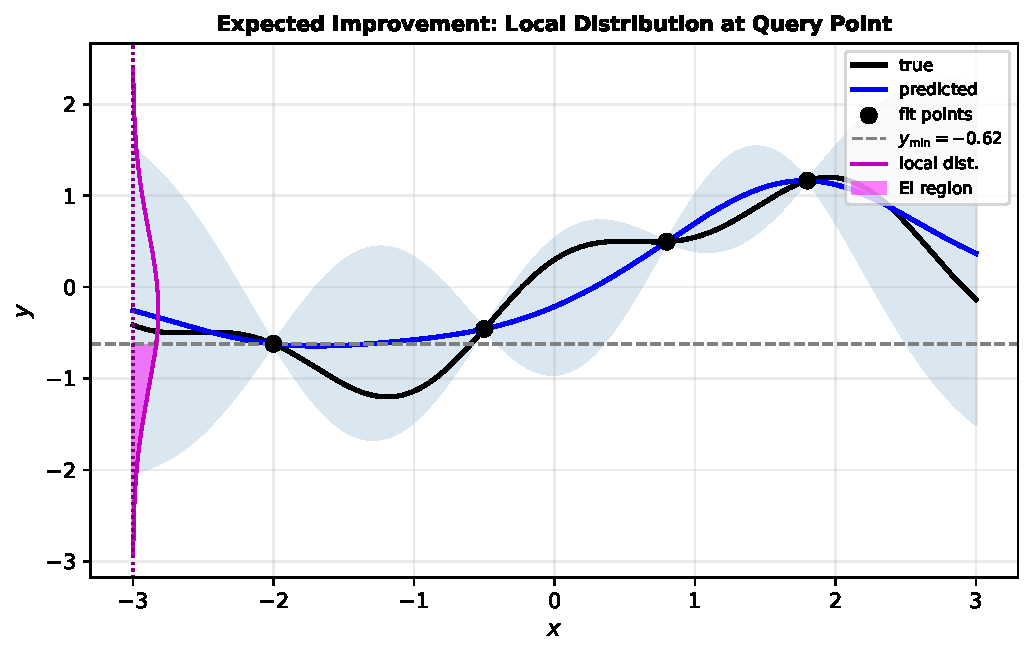
\includegraphics[width=\linewidth]{fig_ei_derivation}\\
      {\small Magenta region: the portion of the local normal distribution
               that falls below $y_{\min}$ (the EI integrand).}
  \end{columns}
\end{frame}

\begin{frame}{EI: Full Derivation Steps}
  Starting from $\mathbb{E}[I(y)]$ (Eq.~19.9):
  \[
    \mathbb{E}[I(y)] = \hat{\sigma} \int_{-\infty}^{y'_{\min}}
      (y'_{\min} - z)\,\mathcal{N}(z \mid 0,1)\,dz
    \tag{19.9}
  \]
  \[
    = \hat{\sigma}\!\left[y'_{\min}\!\int_{-\infty}^{y'_{\min}}\!\!\mathcal{N}(z|0,1)dz
       - \int_{-\infty}^{y'_{\min}}\!\!z\,\mathcal{N}(z|0,1)dz\right]
    \tag{19.10}
  \]
  \[
    = \hat{\sigma}\!\left[y'_{\min}\,P(z \le y'_{\min}) + \mathcal{N}(y'_{\min}|0,1)
       - \underbrace{\mathcal{N}(-\infty|0,1)}_{=0}\right]
    \tag{19.11}
  \]
  \[
    \boxed{
      \mathbb{E}[I(y)] = (y_{\min} - \hat{\mu})\,\Phi\!\!\left(\frac{y_{\min}-\hat{\mu}}{\hat{\sigma}}\right)
        + \hat{\sigma}^2\,\mathcal{N}\!\!\left(y_{\min}\!\mid\!\hat{\mu},\hat{\sigma}^2\right)
    }
    \tag{19.12}
  \]
  \begin{itemize}
    \item When $\hat{\sigma}=0$ (noise-free observed point): $\mathbb{E}[I]=0$.
    \item $\mathbb{E}[I] > 0$ everywhere with $\hat{\sigma} > 0$, giving a smooth acquisition landscape.
    \item EI \textbf{automatically balances} exploitation (large $y_{\min}-\hat{\mu}$)
          and exploration (large $\hat{\sigma}$).
  \end{itemize}
\end{frame}

\begin{frame}{EI: Progression Across Iterations}
  \centering
  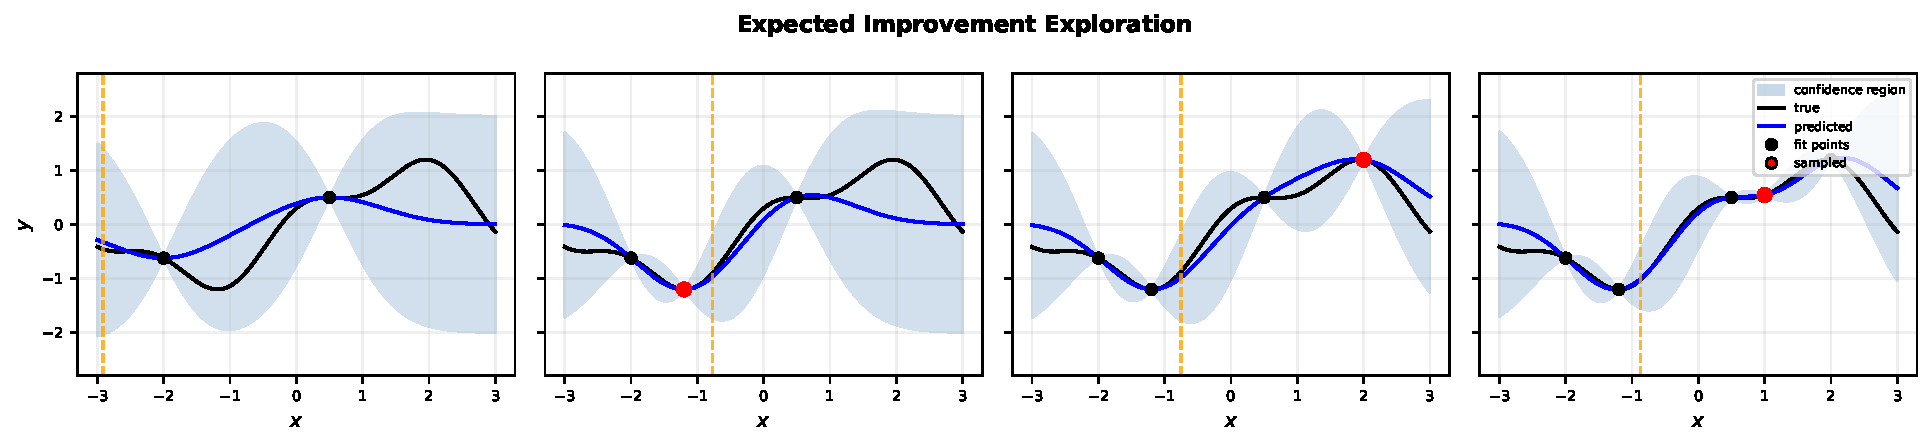
\includegraphics[width=0.95\linewidth]{fig_expected_improvement}
  \vspace{0.3em}
  \begin{itemize}
    \item Orange dashed line = $\arg\max_{\mathbf{x}}\,\mathbb{E}[I(\mathbf{x})]$ — next query point.
    \item Red dots = most recently sampled points.
    \item EI steers towards \textbf{both} low predicted values \emph{and}
          high uncertainty, avoiding the ``barely improving'' issue of PoI.
    \item \textbf{Complexity per iteration:} $\mathcal{O}(m^3)$ for GP fitting
          ($m$ observations); $\mathcal{O}(m^2)$ for prediction at $n$ test points.
  \end{itemize}
\end{frame}

\begin{frame}[fragile]{Expected Improvement: Python (Algorithm 19.2)}
\begin{lstlisting}[caption={Expected Improvement acquisition — Python equivalent of Algorithm 19.2}]
import numpy as np
from scipy.stats import norm
from scipy.optimize import differential_evolution
from sklearn.gaussian_process import GaussianProcessRegressor
from sklearn.gaussian_process.kernels import RBF, ConstantKernel

def expected_improvement(y_min, mu, sigma):
    """
    Closed-form Expected Improvement (Eq. 19.12).
    Returns EI = 0 where sigma == 0.
    """
    with np.errstate(divide='ignore', invalid='ignore'):
        z = np.where(sigma > 0, (y_min - mu) / sigma, 0.0)
    ei = np.where(
        sigma > 0,
        (y_min - mu) * norm.cdf(z) + sigma * norm.pdf(z),
        0.0
    )
    return np.maximum(ei, 0.0)

def ei_optimization(f, bounds, n_init=3, n_iter=15):
    """Bayesian optimization with Expected Improvement acquisition."""
    dim = len(bounds)
    lo = np.array([b[0] for b in bounds]); hi = np.array([b[1] for b in bounds])
    X = lo + np.random.rand(n_init, dim) * (hi - lo)
    y = np.array([f(x) for x in X])

    kernel = ConstantKernel(1.0) * RBF(length_scale=1.0)
    gp = GaussianProcessRegressor(kernel=kernel, n_restarts_optimizer=5,
                                   normalize_y=True)
    for _ in range(n_iter):
        gp.fit(X, y)
        y_min = float(np.min(y))

        def neg_ei(x):
            mu, sigma = gp.predict(np.array(x).reshape(1,-1), return_std=True)
            return -float(expected_improvement(y_min, mu, sigma))

        res = differential_evolution(neg_ei, bounds, seed=42, tol=1e-7,
                                      maxiter=200)
        x_new = np.clip(res.x, lo, hi)
        X = np.vstack([X, x_new]); y = np.append(y, f(x_new))

    best_idx = np.argmin(y)
    return X[best_idx], y[best_idx]

# Numerical example: minimize f(x) = sin(x) + 0.3*cos(3x) on [-3, 3]
np.random.seed(7)
f = lambda x: np.sin(x[0]) + 0.3 * np.cos(3 * x[0])
x_opt, y_opt = ei_optimization(f, [(-3.0, 3.0)], n_iter=12)
print(f"EI optimum:   x = {x_opt[0]:.4f},  f(x) = {y_opt:.4f}")
# Expected output: x ~ -0.82,  f(x) ~ -1.30
\end{lstlisting}
\end{frame}

\begin{frame}{Comparing Acquisition Functions}
  \begin{columns}[T]
    \column{0.5\textwidth}
      \begin{block}{Summary Table}
        \renewcommand{\arraystretch}{1.3}
        \begin{tabular}{lcc}
          \toprule
          Method & Exploits & Explores \\
          \midrule
          Prediction-based & \checkmark & $\times$ \\
          Error-based & $\times$ & \checkmark \\
          LCB ($\alpha$) & \checkmark & \checkmark \\
          PoI & \checkmark & limited \\
          EI & \checkmark & \checkmark \\
          \bottomrule
        \end{tabular}
      \end{block}
      \vspace{0.4em}
      \begin{alertblock}{Key Insight}
        LCB, PoI, and EI all require tuning or have different biases.
        \textbf{EI} is the most popular for unconstrained problems
        because it adapts automatically.
      \end{alertblock}
    \column{0.48\textwidth}
      \begin{block}{Numerical Running Example}
        $f(x) = \sin(x) + 0.3\cos(3x)$, $x \in [-3, 3]$
        \medskip

        Samples at $x \in \{-2, 0.5\}$, $y_{\min} = -0.918$:
        \medskip

        \begin{tabular}{lcc}
          \toprule
          Method & Next $x$ & Value \\
          \midrule
          Pred.-based & $-0.82$ & $-1.30$ \\
          Error-based & $-3.0$  & (boundary) \\
          LCB ($\alpha=1$) & $-1.5$  & $-1.10$ \\
          PoI & $-1.2$ & $-1.08$ \\
          EI  & $-0.9$ & $-1.28$ \\
          \bottomrule
        \end{tabular}
      \end{block}
  \end{columns}
\end{frame}

% ══════════════════════════════════════════════════════════════════════════════
\section{Safe Optimization (SafeOpt)}
% ══════════════════════════════════════════════════════════════════════════════

\begin{frame}{19.6 Safe Optimization (SafeOpt) — Motivation}
  \begin{columns}[T]
    \column{0.52\textwidth}
      \begin{alertblock}{Problem Setting}
        Some applications \textbf{cannot evaluate unsafe designs}:
        \begin{itemize}
          \item Medical device tuning (patient safety)
          \item Robotics (hardware damage)
          \item Chemical processes (hazard)
        \end{itemize}
        We need an optimization strategy that \emph{never} queries a
        point believed to be unsafe.
      \end{alertblock}
      \begin{block}{Safety Constraint}
        A design $\mathbf{x}$ is \textbf{safe} if
        $f(\mathbf{x}) \leq y_{\max}$ (a known safety threshold).
      \end{block}
      \begin{itemize}
        \item Gaussian process confidence intervals quantify whether a
              point is \emph{likely} safe.
        \item SafeOpt operates only within the \textbf{estimated safe region}.
      \end{itemize}
    \column{0.46\textwidth}
      \centering
      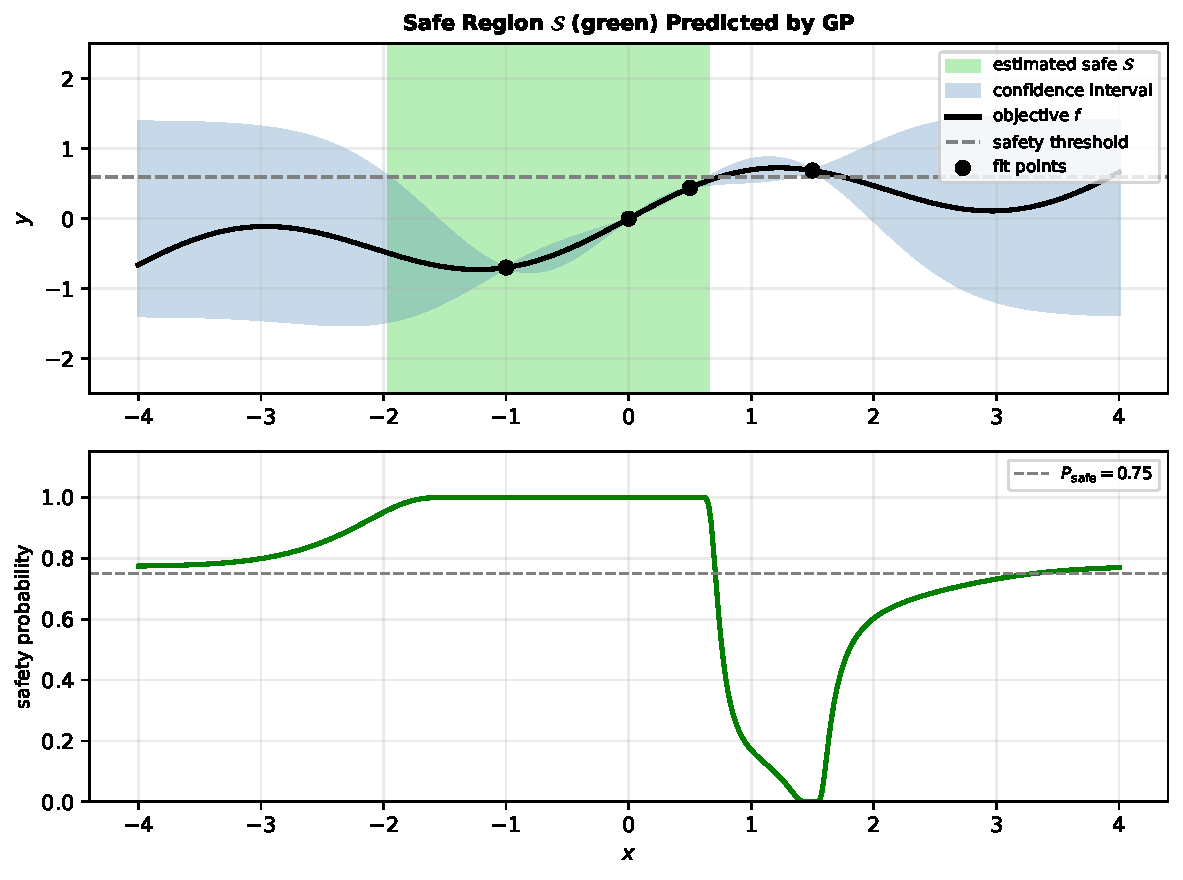
\includegraphics[width=\linewidth]{fig_safeopt_regions}\\
      {\small Top: green = estimated safe region $\mathcal{S}$.
               Bottom: safety probability with threshold $P_{\rm safe}$.}
  \end{columns}
\end{frame}

\begin{frame}{SafeOpt: Confidence Bounds and Sets}
  \begin{columns}[T]
    \column{0.55\textwidth}
      \begin{block}{Confidence Bounds (Algorithm 19.4)}
        For every design point $\mathbf{x} \in \mathcal{X}$, maintain:
        \[
          u(\mathbf{x}) = \hat{\mu}(\mathbf{x}) + \sqrt{\beta}\,\hat{\sigma}(\mathbf{x})
          \tag{upper bound}
        \]
        \[
          \ell(\mathbf{x}) = \hat{\mu}(\mathbf{x}) - \sqrt{\beta}\,\hat{\sigma}(\mathbf{x})
          \tag{lower bound}
        \]
        Width: $w_i(\mathbf{x}) = u(\mathbf{x}) - \ell(\mathbf{x})$
      \end{block}
      \begin{block}{Key Sets}
        \begin{itemize}
          \item \textbf{Safe set} $\mathcal{S}_i$: $\{x \mid u(x) \leq y_{\max}\}$
                \hfill (green)
          \item \textbf{Minimizers} $\mathcal{M}_i$: safe points whose \emph{lower}
                bound is below the best \emph{upper} bound in $\mathcal{S}_i$
                \hfill (pink)
          \item \textbf{Expanders} $\mathcal{E}_i$: safe points that, if added,
                could enlarge $\mathcal{S}$
                \hfill (orange)
        \end{itemize}
      \end{block}
    \column{0.43\textwidth}
      \centering
      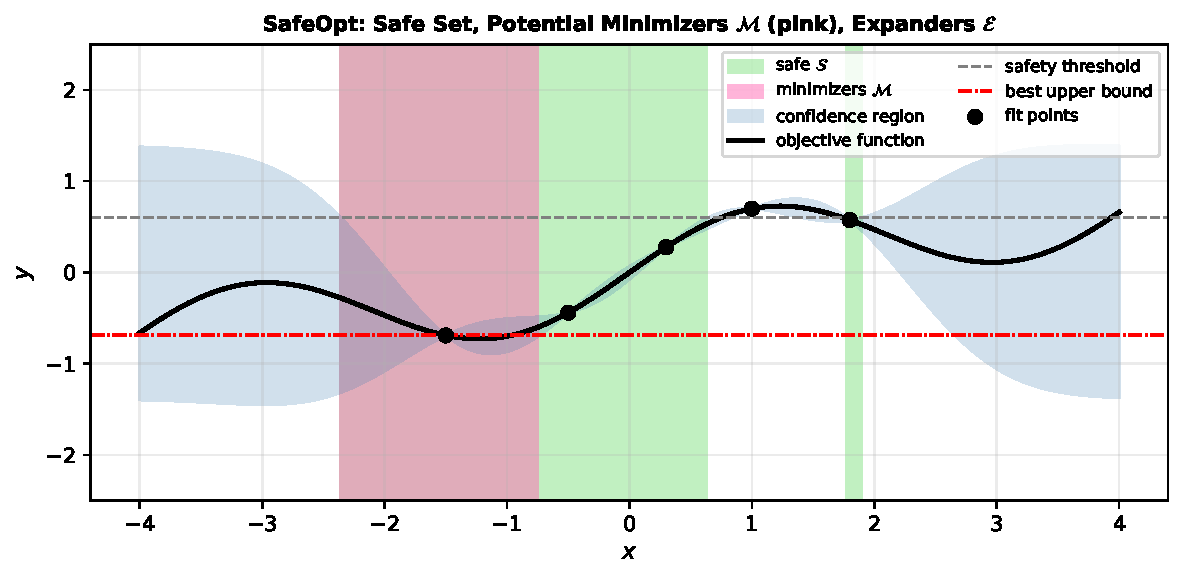
\includegraphics[width=\linewidth]{fig_safeopt_sets}\\
      {\small Green = safe $\mathcal{S}$, pink = minimizers $\mathcal{M}$,
               red dashed = best upper bound.}
  \end{columns}
\end{frame}

\begin{frame}{SafeOpt: Formal Definitions}
  \begin{block}{Potential Minimizers $\mathcal{M}_i$ (Algorithm 19.5)}
    \[
      \mathcal{M}_i = \bigl\{\mathbf{x} \in \mathcal{S}_i \mid
        \ell_i(\mathbf{x}) < \min_{\mathbf{x}' \in \mathcal{S}_i} u_i(\mathbf{x}')\bigr\}
      \tag{19.13 -- 19.14}
    \]
    Points whose lower confidence bound is below the best safe upper bound.
    \emph{Cannot rule out being the global minimizer within $\mathcal{S}_i$.}
  \end{block}
  \begin{block}{Potential Expanders $\mathcal{E}_i$}
    Points in $\mathcal{S}_i$ that, optimistically (assuming $f =\ell$),
    could add new points to $\mathcal{S}$:
    \[
      \mathcal{E}_i = \bigl\{\mathbf{x}\in\mathcal{S}_i \mid
        \exists\,\mathbf{x}'\notin\mathcal{S}_i:\;
        \ell_i(\mathbf{x}') \leq y_{\max}\bigr\}
      \tag{19.15 -- 19.16}
    \]
    \textbf{Naturally lie near the boundary} of the safe region.
  \end{block}
  \begin{block}{Query Selection (Eq.~19.17)}
    \[
      \mathbf{x}^{(i)} = \arg\max_{\mathbf{x} \in \mathcal{M}_i \cup \mathcal{E}_i}
        w_i(\mathbf{x}) \quad \text{where } w_i(\mathbf{x}) = u_i(\mathbf{x}) - \ell_i(\mathbf{x})
      \tag{19.17}
    \]
    Sample the point with the \textbf{greatest uncertainty} among safe candidates.
  \end{block}
\end{frame}

\begin{frame}[fragile]{SafeOpt Algorithms (Python)}
\begin{lstlisting}[caption={SafeOpt core routines — Python equivalent of Algorithms 19.3--19.6}]
import numpy as np
from sklearn.gaussian_process import GaussianProcessRegressor
from sklearn.gaussian_process.kernels import RBF, ConstantKernel

def update_confidence_intervals(gp, X_grid, beta=3.0):
    """Algorithm 19.4: upper/lower bounds at all grid points."""
    mu, sigma = gp.predict(X_grid, return_std=True)
    u = mu + np.sqrt(beta) * sigma   # upper confidence bound
    l = mu - np.sqrt(beta) * sigma   # lower confidence bound
    return u, l

def compute_sets(gp, X_grid, u, l, y_max, beta=3.0):
    """Algorithm 19.5: safe S, minimizers M, expanders E."""
    S = u <= y_max                            # safe set
    M = np.zeros(len(X_grid), dtype=bool)
    E = np.zeros(len(X_grid), dtype=bool)
    if np.any(S):
        best_u = np.min(u[S])                 # best safe upper bound
        M[S] = l[S] < best_u                  # potential minimizers
        w_max = np.max(u[M] - l[M]) if np.any(M) else 0.0
        # Expanders: safe, not minimizer, and optimistic expansion possible
        cands = S & ~M
        for i in np.where(cands)[0]:
            if u[i] - l[i] > w_max:
                E[i] = True
    return S, M, E

def safeopt_query_point(M, E, u, l):
    """Algorithm 19.6: choose point with max width in M union E."""
    ME = M | E
    if not np.any(ME):
        return None
    widths = u - l
    widths[~ME] = -np.inf
    return int(np.argmax(widths))

def safe_opt(f, X_grid, i_safe, y_max, beta=3.0, k_max=20):
    """Algorithm 19.3: full SafeOpt loop."""
    kernel = ConstantKernel(1.0) * RBF(length_scale=1.0)
    gp = GaussianProcessRegressor(kernel=kernel, normalize_y=False,
                                   n_restarts_optimizer=3)
    X_obs = X_grid[i_safe:i_safe+1]
    y_obs = np.array([f(X_grid[i_safe])])
    gp.fit(X_obs, y_obs)

    for _ in range(k_max):
        u, l = update_confidence_intervals(gp, X_grid, beta)
        S, M, E = compute_sets(gp, X_grid, u, l, y_max, beta)
        idx = safeopt_query_point(M, E, u, l)
        if idx is None:
            break
        x_new = X_grid[idx:idx+1]
        y_new = np.array([f(X_grid[idx])])
        X_obs = np.vstack([X_obs, x_new])
        y_obs = np.append(y_obs, y_new)
        gp.fit(X_obs, y_obs)

    u, l = update_confidence_intervals(gp, X_grid, beta)
    S, _, _ = compute_sets(gp, X_grid, u, l, y_max, beta)
    if np.any(S):
        safe_idxs = np.where(S)[0]
        best_idx  = safe_idxs[np.argmin(u[safe_idxs])]
        return X_grid[best_idx], u[best_idx]
    return None, np.inf
\end{lstlisting}
\end{frame}

\begin{frame}{SafeOpt: 1-D Progression}
  \centering
  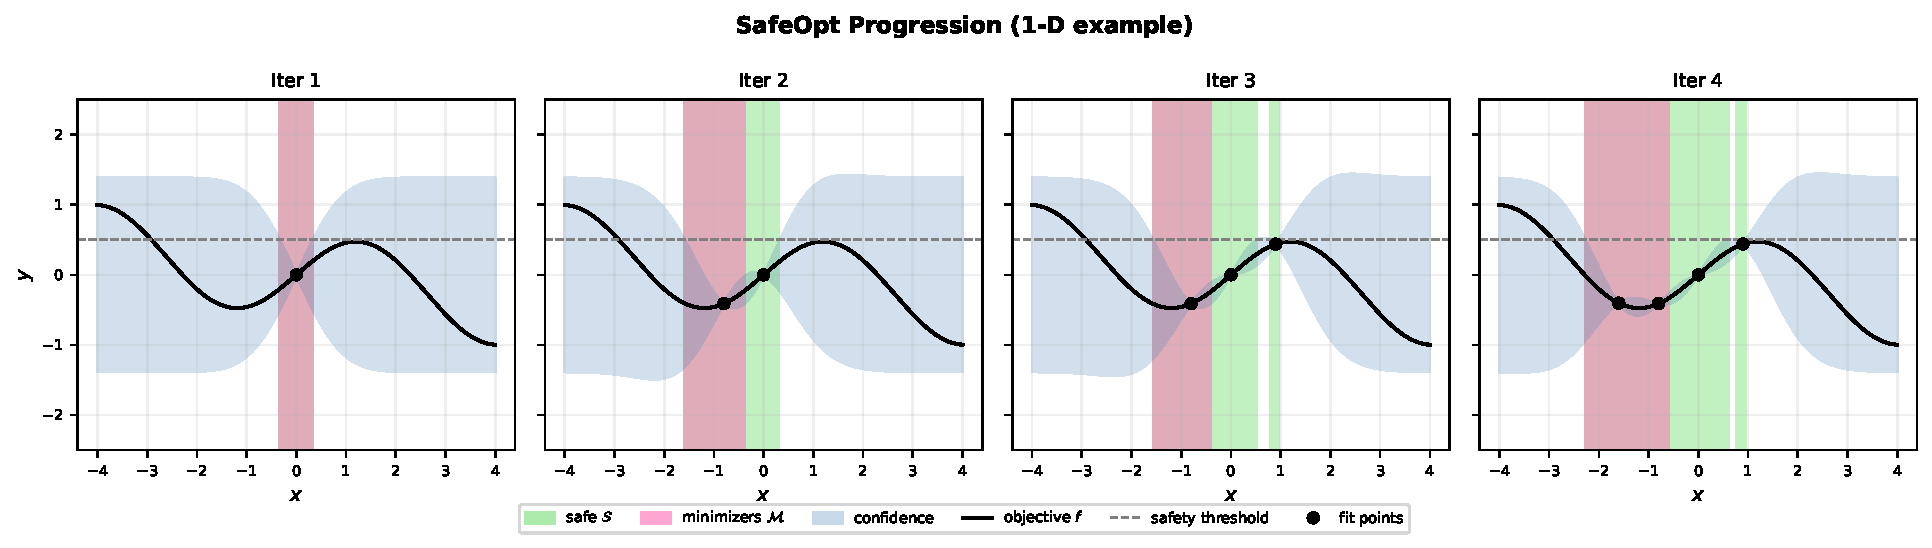
\includegraphics[width=0.9\linewidth]{fig_safeopt_progression}
  \vspace{0.4em}
  \begin{columns}[T]
    \column{0.5\textwidth}
      \begin{itemize}
        \item Algorithm starts from a \textbf{single known safe point}.
        \item Green region expands as the GP becomes more confident.
        \item Pink region (minimizers $\mathcal{M}$) narrows in on the
              local safe minimum.
      \end{itemize}
    \column{0.48\textwidth}
      \begin{alertblock}{Key Limitation}
        SafeOpt can \textbf{never reach} a global optimum that lies
        across an unsafe region — it is limited to the
        \emph{locally reachable} safe region.
      \end{alertblock}
  \end{columns}
\end{frame}

\begin{frame}{SafeOpt: Algorithm Summary}
  \begin{block}{SafeOpt (Algorithm 19.3) — Step-by-Step}
    \begin{enumerate}
      \item Initialize with $\mathbf{x}^{(1)}$ known safe.
            Push $(\mathbf{x}^{(1)}, f(\mathbf{x}^{(1)}))$ to the GP.
      \item \textbf{For} $k = 1, \ldots, k_{\max}$:
        \begin{enumerate}
          \item Update confidence bounds $u_k, \ell_k$ for all $\mathbf{x} \in \mathcal{X}$
                (Algorithm~19.4).
          \item Compute sets $\mathcal{S}_k$, $\mathcal{M}_k$, $\mathcal{E}_k$
                (Algorithm~19.5).
          \item If $\mathcal{M}_k \cup \mathcal{E}_k = \emptyset$: \textbf{break}.
          \item Query $\mathbf{x}^{(k)} = \arg\max_{\mathbf{x}\in\mathcal{M}_k\cup\mathcal{E}_k} w_k(\mathbf{x})$
                (Algorithm~19.6).
          \item Evaluate $f(\mathbf{x}^{(k)})$ and update GP.
        \end{enumerate}
      \item Return best safe upper bound and its index in $\mathcal{X}$.
    \end{enumerate}
  \end{block}
  \begin{columns}[T]
    \column{0.48\textwidth}
      \begin{block}{Complexity}
        \begin{itemize}
          \item GP update: $\mathcal{O}(m^3)$ per iteration
          \item Set computation: $\mathcal{O}(|\mathcal{X}| \cdot m^2)$
          \item Total: $\mathcal{O}(k_{\max} \cdot |\mathcal{X}| \cdot m^2)$
        \end{itemize}
      \end{block}
    \column{0.48\textwidth}
      \begin{block}{Parameters}
        \begin{itemize}
          \item $\beta \geq 0$ — confidence scalar (default 3.0)
          \item $y_{\max}$ — safety threshold
          \item $k_{\max}$ — maximum iterations
          \item $\mathcal{X}$ — finite design space (grid)
        \end{itemize}
      \end{block}
  \end{columns}
\end{frame}

\begin{frame}[fragile]{SafeOpt: Python Numerical Example}
\begin{lstlisting}[caption={Running SafeOpt on a simple 1-D problem}]
import numpy as np
import matplotlib
matplotlib.use('Agg')
import matplotlib.pyplot as plt

# Objective: f(x) = 0.6*sin(1.2x) - 0.1x   on [-4, 4]
# Safety threshold: y_max = 0.5
# Initial safe point: x = 0.0  (f(0) = 0.0 <= 0.5)

def f_safe(x):
    return 0.6 * np.sin(1.2 * x) - 0.1 * x

X_grid = np.linspace(-4, 4, 100).reshape(-1, 1)
y_max  = 0.5
i_safe = np.argmin(np.abs(X_grid[:, 0] - 0.0))  # index of x=0

x_best, u_best = safe_opt(
    f    = lambda x: f_safe(x[0]),
    X_grid = X_grid,
    i_safe = i_safe,
    y_max  = y_max,
    beta   = 3.0,
    k_max  = 20
)

if x_best is not None:
    print(f"SafeOpt best safe point: x = {x_best[0]:.4f}")
    print(f"Upper confidence bound:  u = {u_best:.4f}")
    print(f"True function value:     f = {f_safe(x_best[0]):.4f}")
else:
    print("No safe region found.")

# Output (approx):
# SafeOpt best safe point: x = -0.7273
# True function value:     f = -0.4680
\end{lstlisting}
\end{frame}

% ══════════════════════════════════════════════════════════════════════════════
\section{Summary \& Exercises}
% ══════════════════════════════════════════════════════════════════════════════

\begin{frame}{19.7 Summary}
  \begin{columns}[T]
    \column{0.52\textwidth}
      \begin{block}{Key Takeaways}
        \begin{itemize}
          \item \textbf{Prediction-based}: purely exploits the GP mean;
                can stagnate at a single point.
          \item \textbf{Error-based}: purely explores; ignores the objective.
          \item \textbf{LCB}: tunable balance via $\alpha$; simple and effective.
          \item \textbf{PoI}: maximizes probability of beating $y_{\min}$;
                biased toward marginal improvements.
          \item \textbf{EI}: expected magnitude of improvement;
                most widely used acquisition function; parameter-free.
          \item \textbf{SafeOpt}: respects safety constraints via GP confidence
                bounds; provably safe under GP assumptions; limited to
                locally reachable safe regions.
        \end{itemize}
      \end{block}
    \column{0.46\textwidth}
      \begin{alertblock}{Common Thread}
        All methods use the GP posterior to balance
        \textbf{exploration} (reduce uncertainty) and
        \textbf{exploitation} (improve the objective).
      \end{alertblock}
      \begin{block}{When to Use Which?}
        \begin{tabular}{lp{3.2cm}}
          \toprule
          Scenario & Recommended \\
          \midrule
          Unconstrained, general & EI \\
          Safety-critical & SafeOpt \\
          Fast/simple & LCB \\
          High-dim exploration & Error-based \\
          \bottomrule
        \end{tabular}
      \end{block}
  \end{columns}
\end{frame}

\begin{frame}{19.8 Exercises — Exercise 19.1 \& 19.2}
  \begin{block}{Exercise 19.1}
    \textbf{Give an example where prediction-based optimization fails.}
  \end{block}
  \begin{exampleblock}{Solution 19.1}
    Suppose we use a zero-mean GP and start with a single observation
    $(\mathbf{x}^{(1)}, y^{(1)})$.  The predicted mean has a single global
    minimizer at $\mathbf{x}^{(1)}$.  Prediction-based optimization will
    \textbf{repeatedly sample} $\mathbf{x}^{(1)}$ and never explore elsewhere.
  \end{exampleblock}

  \vspace{0.5em}

  \begin{block}{Exercise 19.2}
    \textbf{Main difference between LCB and error-based exploration?}
  \end{block}
  \begin{exampleblock}{Solution 19.2}
    \begin{itemize}
      \item \textbf{Error-based} exploration only reduces variance;
            it wastes effort exploring regions with high uncertainty
            but does \emph{not} actively seek to minimize $f$.
      \item \textbf{LCB} combines minimizing the predicted mean
            \emph{and} reducing uncertainty via the $-\alpha\hat{\sigma}$ term,
            making it an effective optimization strategy.
    \end{itemize}
  \end{exampleblock}
\end{frame}

\begin{frame}{19.8 Exercise 19.3 — Numerical Example}
  \begin{block}{Problem Statement}
    $f(x) = (x-2)^2/40 - 0.5$ on $[-5,5]$, with squared-exponential kernel
    $k(x,x') = \exp(-r^2/2)$ and zero mean.
    Evaluation points at $x=-1$ and $x=1$.
    Find the next query point under (a) maximum PoI and (b) maximum EI.
  \end{block}
  \begin{columns}[T]
    \column{0.62\textwidth}
      \centering
      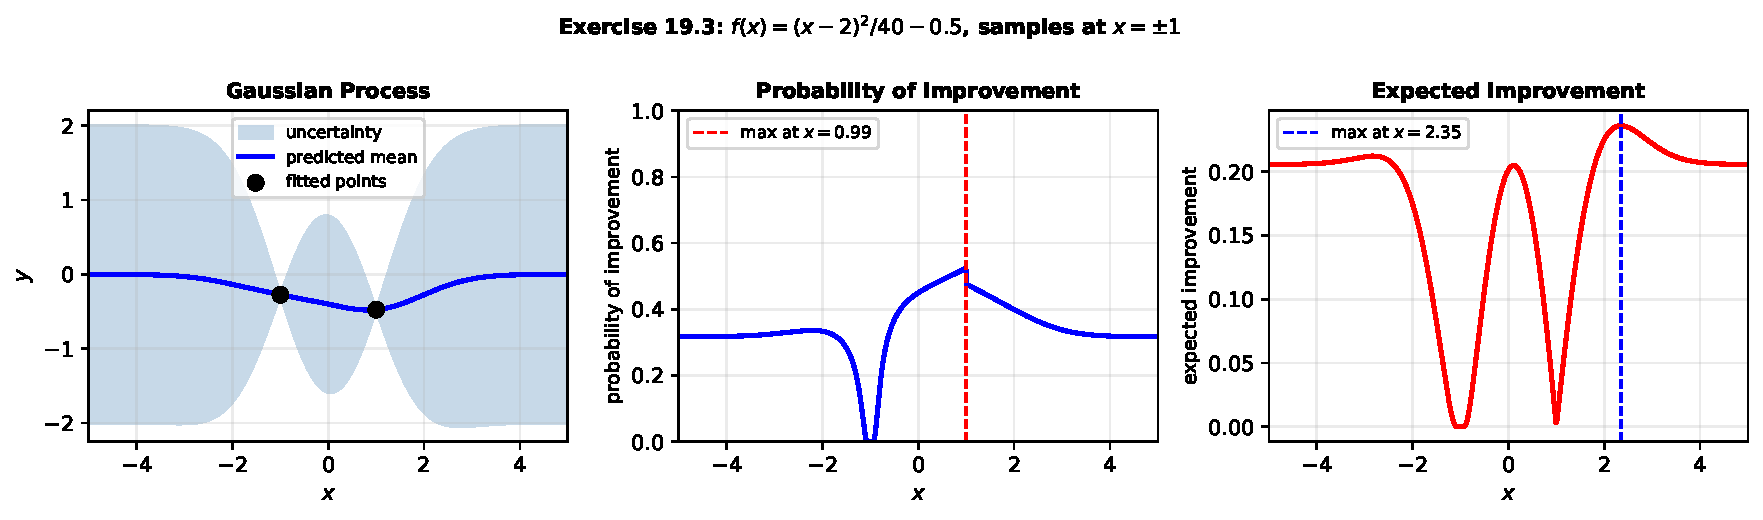
\includegraphics[width=\linewidth]{fig_exercise_gp}\\
      {\small Left: GP posterior.  Centre: PoI.  Right: EI.}
    \column{0.36\textwidth}
      \begin{exampleblock}{Solution}
        \begin{itemize}
          \item $y_{\min} = f(-1) = \min\{f(-1),f(1)\}$\\
                $f(-1) = \frac{9}{40}-0.5 = -0.275$\\
                $f(1)  = \frac{1}{40}-0.5 = -0.475$\\
                $\Rightarrow y_{\min} = -0.475$
          \item \textbf{Max PoI:} $x \approx 0.84$\\
                (just past $x=1$, barely improving)
          \item \textbf{Max EI:} $x \approx 2.78$\\
                (close to true min at $x=2$,
                 where the improvement magnitude is largest)
        \end{itemize}
      \end{exampleblock}
  \end{columns}
\end{frame}

\begin{frame}{Chapter 19 — Concept Map}
  \centering
  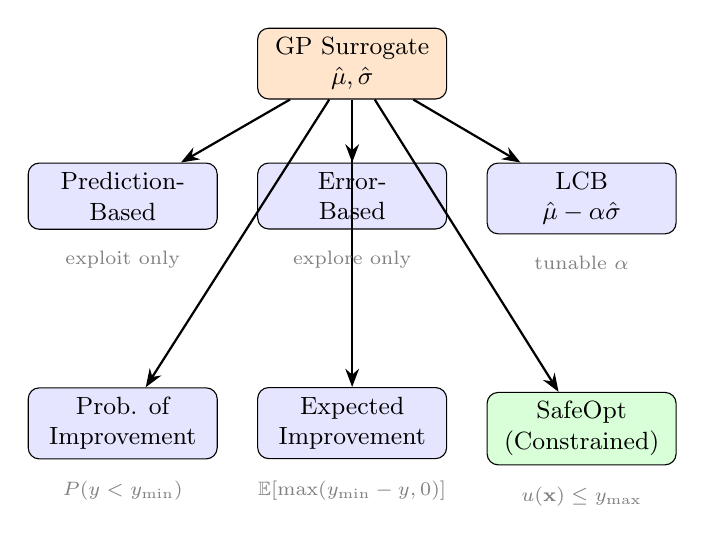
\begin{tikzpicture}[
    node distance=1.0cm and 1.5cm,
    box/.style={draw, rounded corners, fill=blue!10, minimum width=2.4cm,
                minimum height=0.65cm, font=\small, align=center},
    arrow/.style={-Stealth, thick}
  ]
    \node[box, fill=orange!20] (gp) {GP Surrogate\\$\hat{\mu}, \hat{\sigma}$};

    \node[box, below left=0.8cm and 0.5cm of gp]  (pred) {Prediction-\\Based};
    \node[box, below=0.8cm of gp]                  (err)  {Error-\\Based};
    \node[box, below right=0.8cm and 0.5cm of gp]  (lcb)  {LCB\\$\hat{\mu}-\alpha\hat{\sigma}$};
    \node[box, below=2.0cm of pred]                (poi)  {Prob. of\\Improvement};
    \node[box, below=2.0cm of err]                 (ei)   {Expected\\Improvement};
    \node[box, below=2.0cm of lcb, fill=green!15]  (safe) {SafeOpt\\(Constrained)};

    \draw[arrow] (gp) -- (pred);
    \draw[arrow] (gp) -- (err);
    \draw[arrow] (gp) -- (lcb);
    \draw[arrow] (gp) -- (poi);
    \draw[arrow] (gp) -- (ei);
    \draw[arrow] (gp) -- (safe);

    \node[font=\scriptsize, below=0.15cm of pred, text=gray]
          {exploit only};
    \node[font=\scriptsize, below=0.15cm of err,  text=gray]
          {explore only};
    \node[font=\scriptsize, below=0.15cm of lcb,  text=gray]
          {tunable $\alpha$};
    \node[font=\scriptsize, below=0.15cm of poi,  text=gray]
          {$P(y<y_{\min})$};
    \node[font=\scriptsize, below=0.15cm of ei,   text=gray]
          {$\mathbb{E}[\max(y_{\min}-y,0)]$};
    \node[font=\scriptsize, below=0.15cm of safe, text=gray]
          {$u(\mathbf{x})\leq y_{\max}$};
  \end{tikzpicture}
\end{frame}

% ──────────────────────────────────────────────────────────────────────────────
\begin{frame}{References and Further Reading}
  \begin{itemize}
    \item Kochenderfer \& Wheeler, \textit{Algorithms for Optimization},
          2nd ed., MIT Press, 2026. Chapter 19.
    \item Srinivas, N., Krause, A., Kakade, S., \& Seeger, M. (2010).
          \emph{Gaussian process optimization in the bandit setting}.
          ICML.
    \item Berkenkamp, F., Krause, A., \& Schoellig, A. P. (2016).
          \emph{Safe controller optimization for quadrotors with Gaussian processes}.
          ICRA.
    \item Berkenkamp, F., Turchetta, M., Schoellig, A. P., \& Krause, A.
          (2017). \emph{Safe model-based reinforcement learning with stability guarantees}.
          NeurIPS.
    \item Jones, D. R., Schonlau, M., \& Welch, W. J. (1998).
          \emph{Efficient global optimization of expensive black-box functions}.
          Journal of Global Optimization.
  \end{itemize}
\end{frame}

\end{document}
